% ============================================================
%  Rozdział 3 — Locja
% ============================================================
\section{Locja}

% ------------------------------------------------------------
\subsection{Skala oceny trudności}
% ------------------------------------------------------------

\begin{longtable}{>{\bfseries\centering}p{1.8cm}
                  >{\centering}p{2.2cm}
                  p{5.2cm}
                  p{4.2cm}}
  \toprule
  \textbf{Stopień WW} & \textbf{Nazwa} & \textbf{Charakterystyka rzeki}
    & \textbf{Wymagania dla kajakarza} \\
  \midrule
  \endfirsthead
  \toprule
  \textbf{Stopień WW} & \textbf{Nazwa} & \textbf{Charakterystyka rzeki}
    & \textbf{Wymagania dla kajakarza} \\
  \midrule
  \endhead
  \bottomrule
  \endfoot

  WW I & Bardzo łatwa
    & Nurt szybki, ale czytelny; drobne fale; brak istotnych przeszkód. & Podstawowe umiejętności sterowania. \\[4pt]

  WW II & Łatwa & Wyraźne bystrza, małe fale, proste przeszkody; dobra widoczność linii. & Kontrola kajaka, podstawowa technika. \\[4pt]

  WW III & Średnia & Silniejszy nurt, większe fale, progi, odwoje; wymagane manewry. & Dobra technika, pewna eskimoska; linia płynięcia możliwa do odczytania
      z kajaka. \\[4pt]

  WW IV & Trudna & Długie, techniczne bystrza, silne odwoje, ciasne linie. & Bardzo dobra technika, czytanie wody; miejscami konieczne planowanie linii z brzegu; ryzyko kontuzji przy odejściu od zaplanowanej linii. \\[4pt]

  WW V & Bardzo trudna & Duże spadki, wodospady, groźne odwoje i podmycia. & Ekspercka technika, asekuracja, skautowanie z brzegu; odejście od linii niesie ryzyko poważnej kontuzji lub śmierci. \\[4pt]

  WW VI & Ekstremalna & Skrajnie niebezpieczna, praktycznie niepływalna. & Ekspedycje ekstremalne, wielodniowe skautowanie; wysokie ryzyko śmierci. \\
\end{longtable}

% ------------------------------------------------------------
\subsection{Brzeg}
% ------------------------------------------------------------

Krawędź koryta rzeki. Oddziela wodę płynącą od lądu i jest kształtowany przez nurt. Brzeg może być \textbf{prawy} lub \textbf{lewy} — określamy je patrząc \emph{w dół rzeki},
z nurtem. Takie podejście niweluje nieporozumienia w komunikacji kajakarzy. Brzeg bywa miejscem zagrożeń, dlatego nawet znajdując się na nim konieczne jest zachowanie szczególnej ostrożności.

% ------------------------------------------------------------
\subsection{Nurt}
% ------------------------------------------------------------

Kierunek i ruch wody w rzece. Jego siłę i kierunek determinuje ilość wody, kierunek, spadek terenu oraz różne przeszkody w korycie.

% ------------------------------------------------------------
\subsection{Bystrze}
% ------------------------------------------------------------

Odcinek rzeki, na którym następuje przyspieszenie nurtu spowodowane wypłyceniem, zwężeniem, spadkiem terenu lub innymi czynnikami. Woda jest wzburzona, nurt rozbija się o kamienie tworząc fale, białe grzywy i prądy. Bystrza zawierają takie elementy jak głazy, cofki, hyżki, odwoje, podmytki, poduszki.

Upraszczając, mają kształt litery „V" rozwartej w górę rzeki — jeśli nie ma większych przeszkód, najlepiej płynąć środkiem.

% ------------------------------------------------------------
\subsection{Zwałka}
% ------------------------------------------------------------

Przeszkoda na rzece do pokonania nad nią lub pod (czasami bez konieczności wysiadania z kajaka). Przykład: przewrócone drzewo.

% ------------------------------------------------------------
\subsection{Cofka}
% ------------------------------------------------------------

Miejsce na rzece z nurtem przeciwnym do głównego nurtu rzeki, często dużo wolniejszym i spokojniejszym. Tworzy się za przeszkodą — kamieniem, gałęzią, drzewem, mielizną, zakrętem itp. Może powstawać przy brzegu lub na środku rzeki.

Jest \textbf{bardzo ważnym elementem rzeki} dla kajakarza — pełni rolę miejsca do wsiadania lub bezpiecznego opuszczenia kajaka, odpoczynku, rozejrzenia się, obejrzenia dalszego
odcinka, zaplanowania trasy i zebrania grupy.

Nie każda cofka jest bezpieczna — zawsze oceniamy ją samodzielnie. Na co zwrócić uwagę: 

\begin{itemize}[leftmargin=1.5em, itemsep=3pt]
  \item \textbf{Długość cofki} — zbyt krótka może być trudna do złapania lub może wymyć kajakarza, zmuszając go do dalszego płynięcia. 
  \item \textbf{Szerokość cofki} — dobrze, jeśli jest przynajmniej tak szeroka, że kajak obróci się w niej w osi poziomej o 360°.
  \item \textbf{Pulsacja wody} — gdy woda pulsuje, zmienia się jej poziom w cofce i trudniej jest się w niej utrzymać; czasem cofka może zniknąć i po chwili pojawić się ponownie.
\end{itemize}

% ------------------------------------------------------------
\subsection{Hyżka}
% ------------------------------------------------------------

Granica między głównym nurtem a cofką. Na samym początku (zaraz za przeszkodą) jest wąska, ale rozszerza się i rozmywa w dół głównego nurtu. Wchodząc do cofki, kajakarzowi zależy
na przecięciu hyżki z odpowiednią prędkością, jak najwyżej / jak najbliżej przeszkody, która tę cofkę tworzy.

\begin{figure}[H]
    \centering
    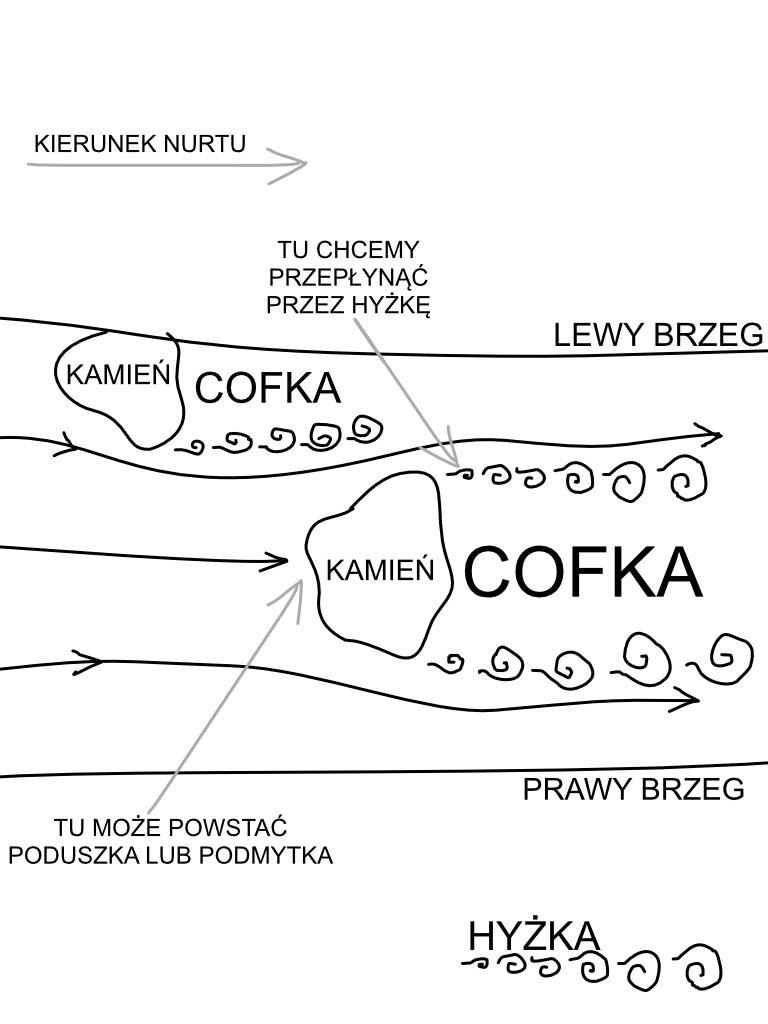
\includegraphics[width=250px]{images/locja.jpg}
    \caption{Opis wybranych elementów rzeki}
\end{figure}

% ------------------------------------------------------------
\subsection{Odwój}
% ------------------------------------------------------------

Element rzeki powstający poniżej progu, stopnia lub przeszkody, gdzie spadająca woda cofa się w górę rzeki tworząc „wałek" spowalniający. Woda spadająca z progu uderza w taflę lub dno, zawijając się w górę i w kierunku progu.

\subsubsection*{Płytka cyrkulacja}

Wałek, w którym obieg wody zachodzi głównie przy powierzchni. Woda miesza się dynamicznie, ale szybko „puszcza" kajak lub pływaka, wypychając go do przodu. Najczęściej występuje
na naturalnych bystrzach i małych progach. Fala jest głośna, spieniona i wyraźna. Zagrożenie niskie do umiarkowanego; możliwość samodzielnego wypłynięcia duża. \emph{Strategia: zdecydowane przepłynięcie z prędkością.}

\subsubsection*{Głęboka cyrkulacja}

Niebezpieczny wałek z głębokim, zamkniętym obiegiem wody. Silnie wciąga w stronę dna i może wielokrotnie „prać" pływaka, utrudniając wydostanie się. Często występuje poniżej
sztucznych progów i zapór. Fala bywa regularna i pozornie spokojna. Zagrożenie wysokie; możliwość samodzielnego wypłynięcia bardzo mała. \emph{Strategia: omijanie lub przenoska.}

\vspace{0.5em}
\noindent
\begin{minipage}[t]{0.48\linewidth}
\begin{tcolorbox}[
  equal height group=odwoj,
  colback=clubgray, colframe=clubblue!60,
  fonttitle=\bfseries\color{white},
  title=Płytka cyrkulacja,
  coltitle=white, colbacktitle=clubblue!60
]
\begin{description}[leftmargin=0pt, labelwidth=\linewidth, font=\bfseries\small]
  \item[Głębokość obiegu:] Głównie przy powierzchni
  \item[Kierunek sił:] Miesza wodę, szybko puszcza
  \item[Zachowanie wody:] Szybko wypycha do przodu
  \item[Wpływ na pływaka:] Chwilowe zatrzymanie
  \item[Możliwość wypłynięcia:] Duża
  \item[Typowe miejsce:] Naturalne bystrza, małe progi
  \item[Charakter fali:] Głośna, spieniona
  \item[Stopień zagrożenia:] Niski–umiarkowany
  \item[Strategia:] Przepłynięcie z prędkością
\end{description}
\end{tcolorbox}
\end{minipage}
\hfill
\begin{minipage}[t]{0.48\linewidth}
\begin{tcolorbox}[
  equal height group=odwoj,
  colback=warnred, colframe=warnframe,
  fonttitle=\bfseries,
  title=Głęboka cyrkulacja,
  coltitle=white, colbacktitle=warnframe
]
\begin{description}[leftmargin=0pt, labelwidth=\linewidth, font=\bfseries\small]
  \item[Głębokość obiegu:] Sięga głęboko pod wodę
  \item[Kierunek sił:] Silne wciąganie w stronę dna
  \item[Zachowanie wody:] Krąży w zamkniętej pętli
  \item[Wpływ na pływaka:] Wielokrotne "pranie"; wciąganie pod wodę
  \item[Możliwość wypłynięcia:] Bardzo mała
  \item[Typowe miejsce:] Sztuczne progi, zapory
  \item[Charakter fali:] Regularna, cicha, bez widocznej grzywy
  \item[Stopień zagrożenia:] Wysoki / śmiertelny
  \item[Strategia:] Omijanie, przenoska
\end{description}
\end{tcolorbox}
\end{minipage}
\vspace{0.5em}

\begin{figure}[H]
  \centering
  \begin{minipage}[t]{0.48\linewidth}
    \centering
    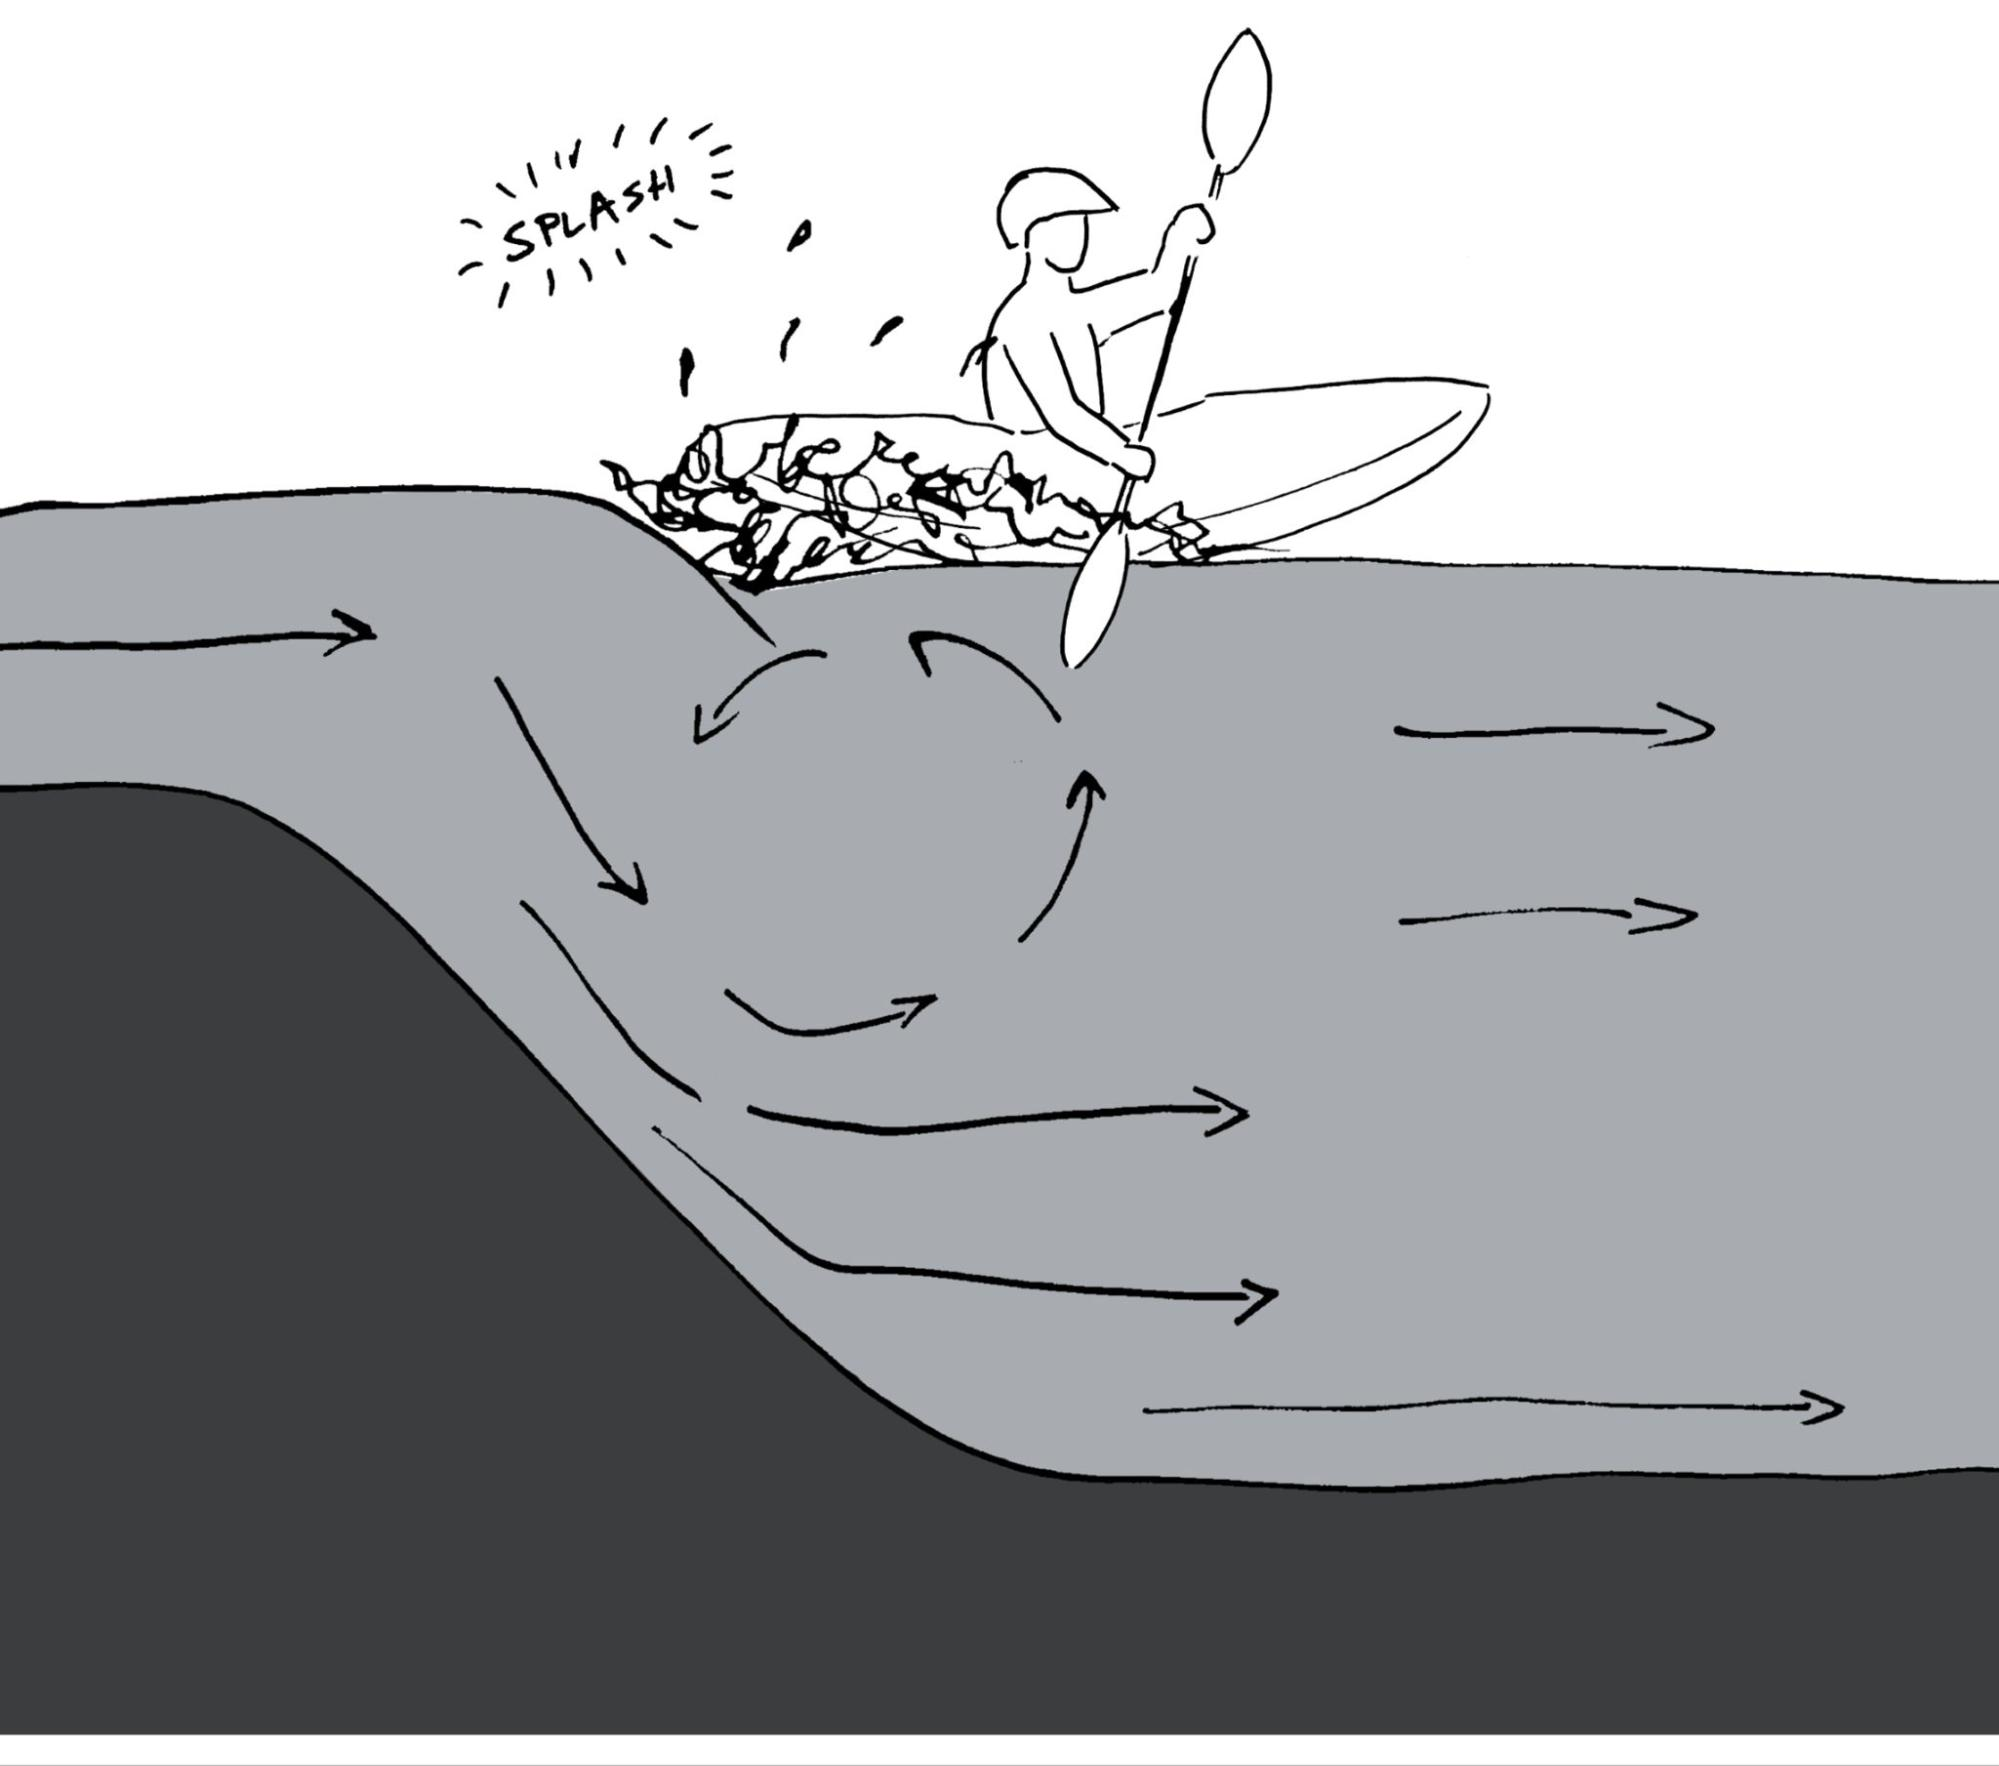
\includegraphics[width=\linewidth]{images/plytki_odwoj.jpg}
    \caption*{(a) Odwój o płytkiej cyrkulacji}
  \end{minipage}
  \hfill
  \begin{minipage}[t]{0.48\linewidth}
    \centering
    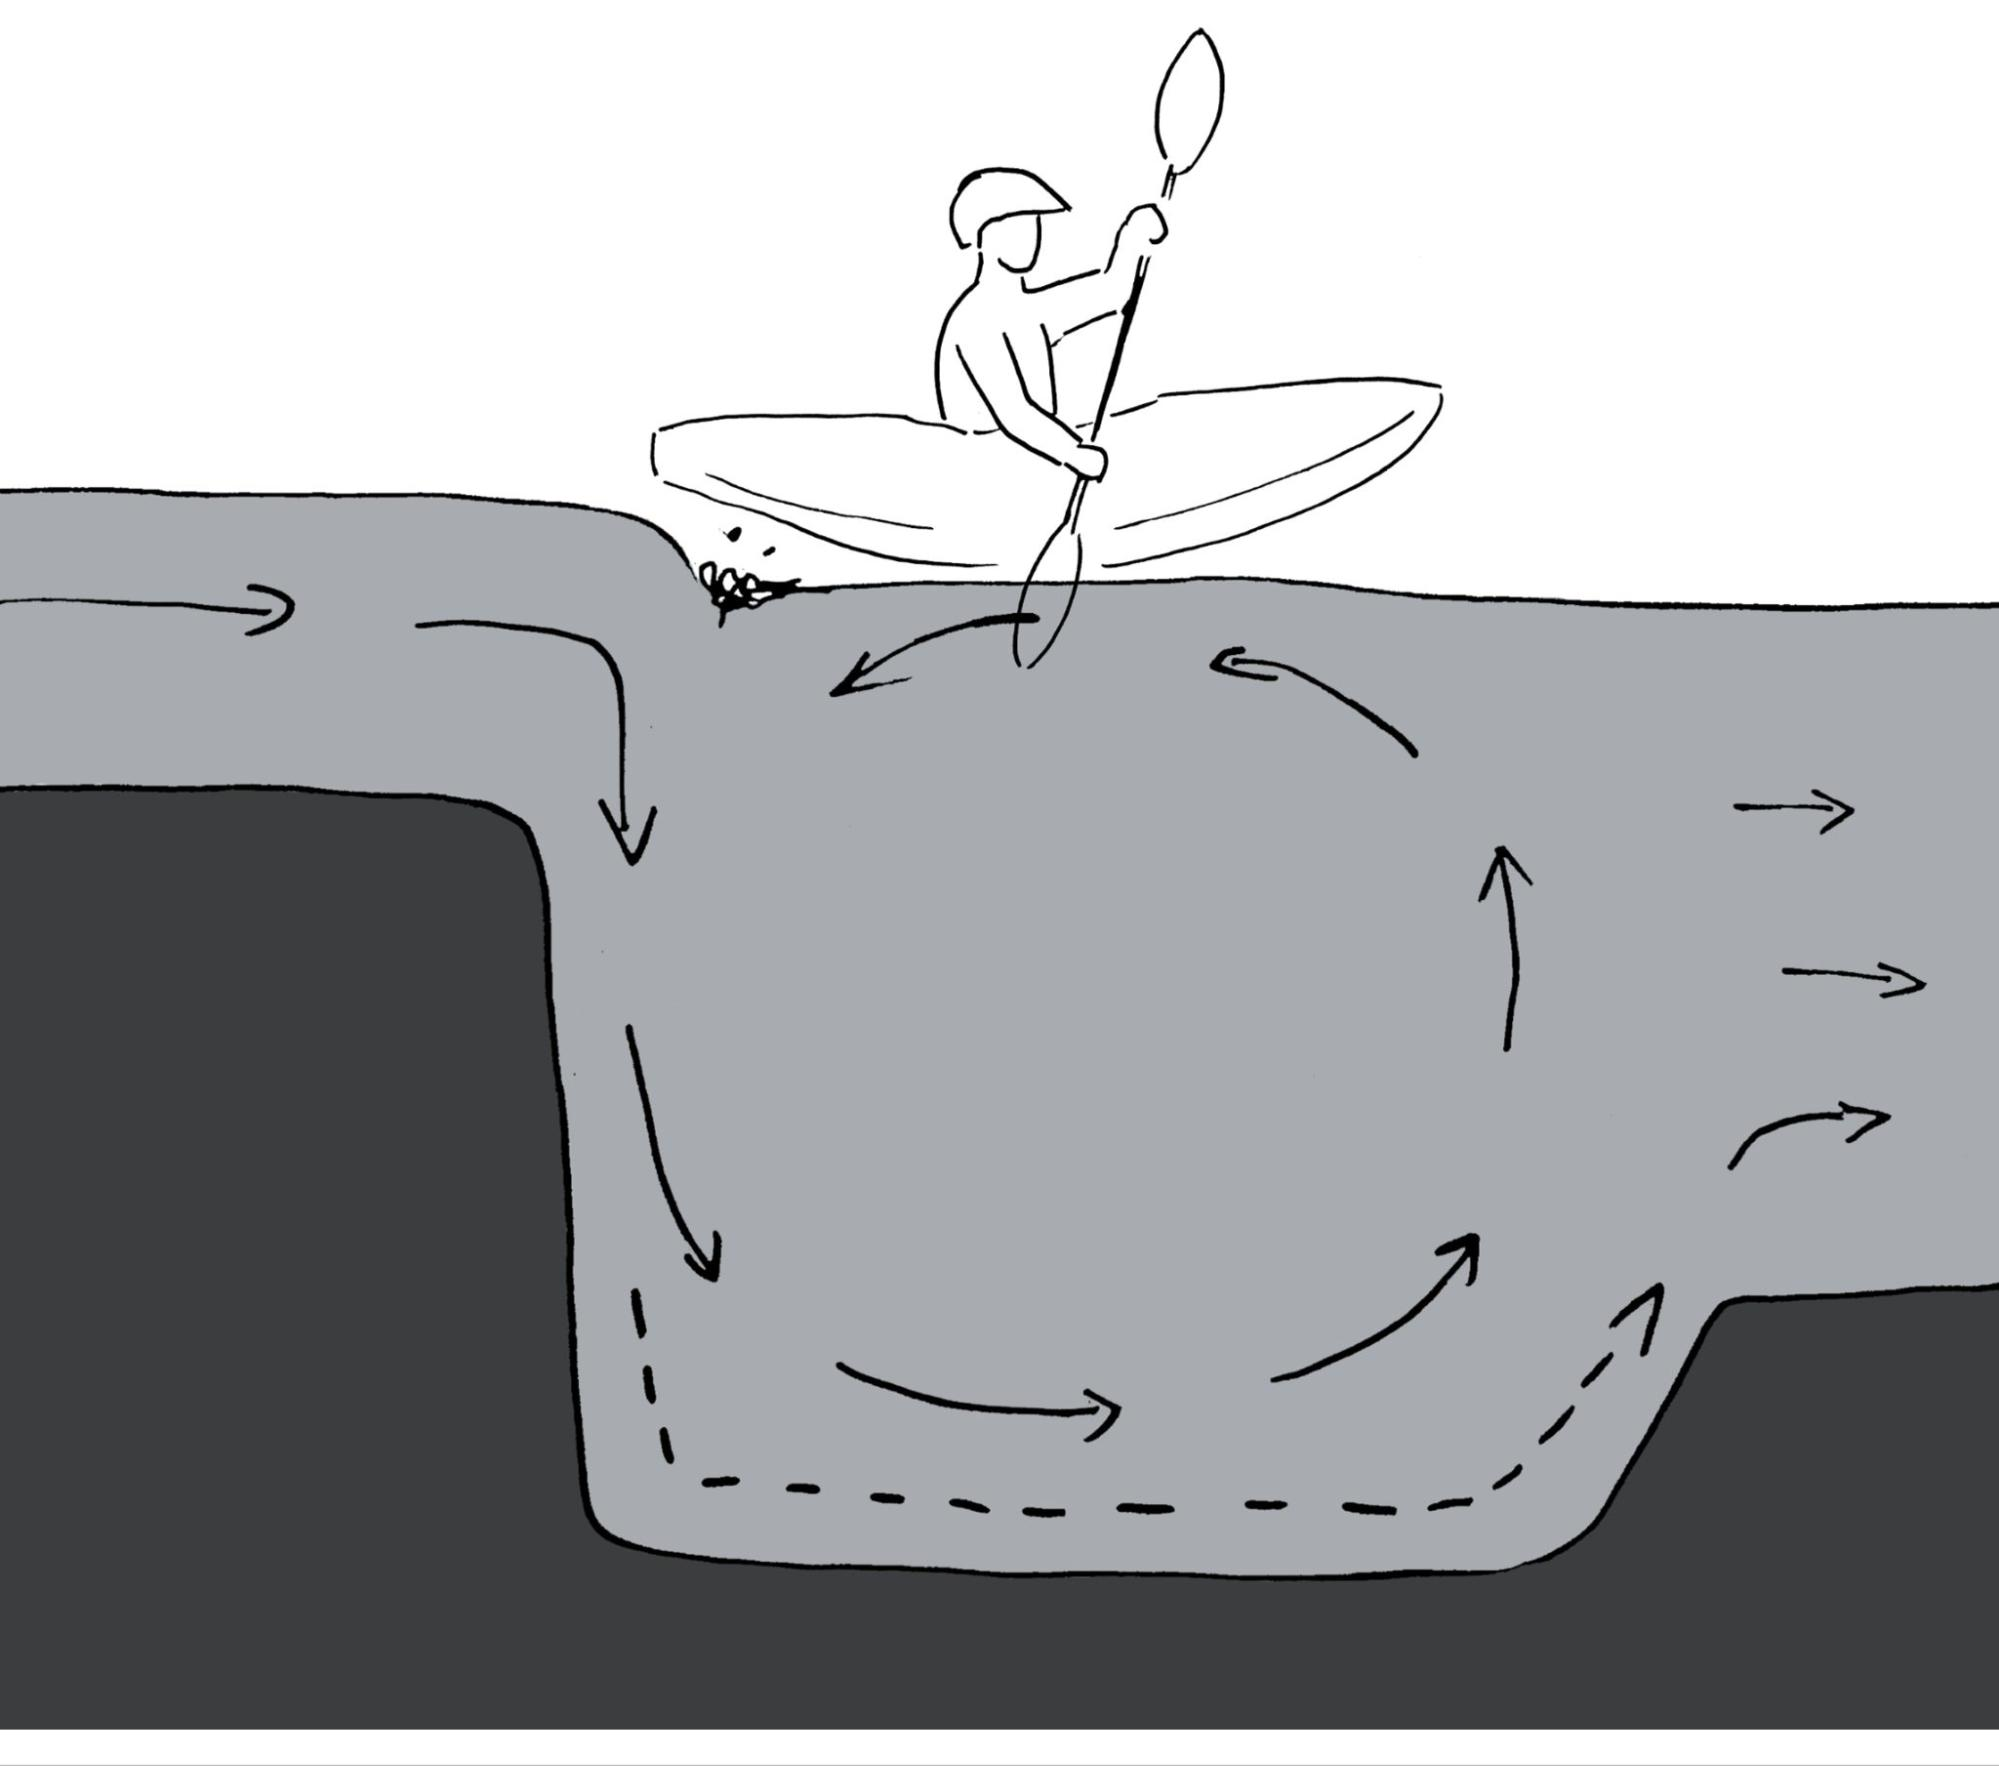
\includegraphics[width=\linewidth]{images/gleboki_odwoj.jpg}
    \caption*{(b) Odwój o głębokiej cyrkulacji}
  \end{minipage}
  \caption{Rodzaje odwojów}
\end{figure}

% ------------------------------------------------------------
\subsection{Podmytka / Syfon}
% ------------------------------------------------------------

Bardzo groźne miejsca na rzece górskiej. Podmytka to przeszkoda (najczęściej kamień, brzeg lub drzewo), pod którą woda przepływa swobodnie, jednak kajakarz może zostać wciągnięty pod nią przez nurt i przyparty do niej bez możliwości przedostania się na drugą stronę ze względu na swoje rozmiary. Podmytka różni się od syfonu tym, że jest z jednej strony otwarta; syfon to miejsce, gdzie nurt przepływa przez otwór w kamieniu bądź między narzuconymi kamieniami.

\begin{figure}[H]
    \centering
    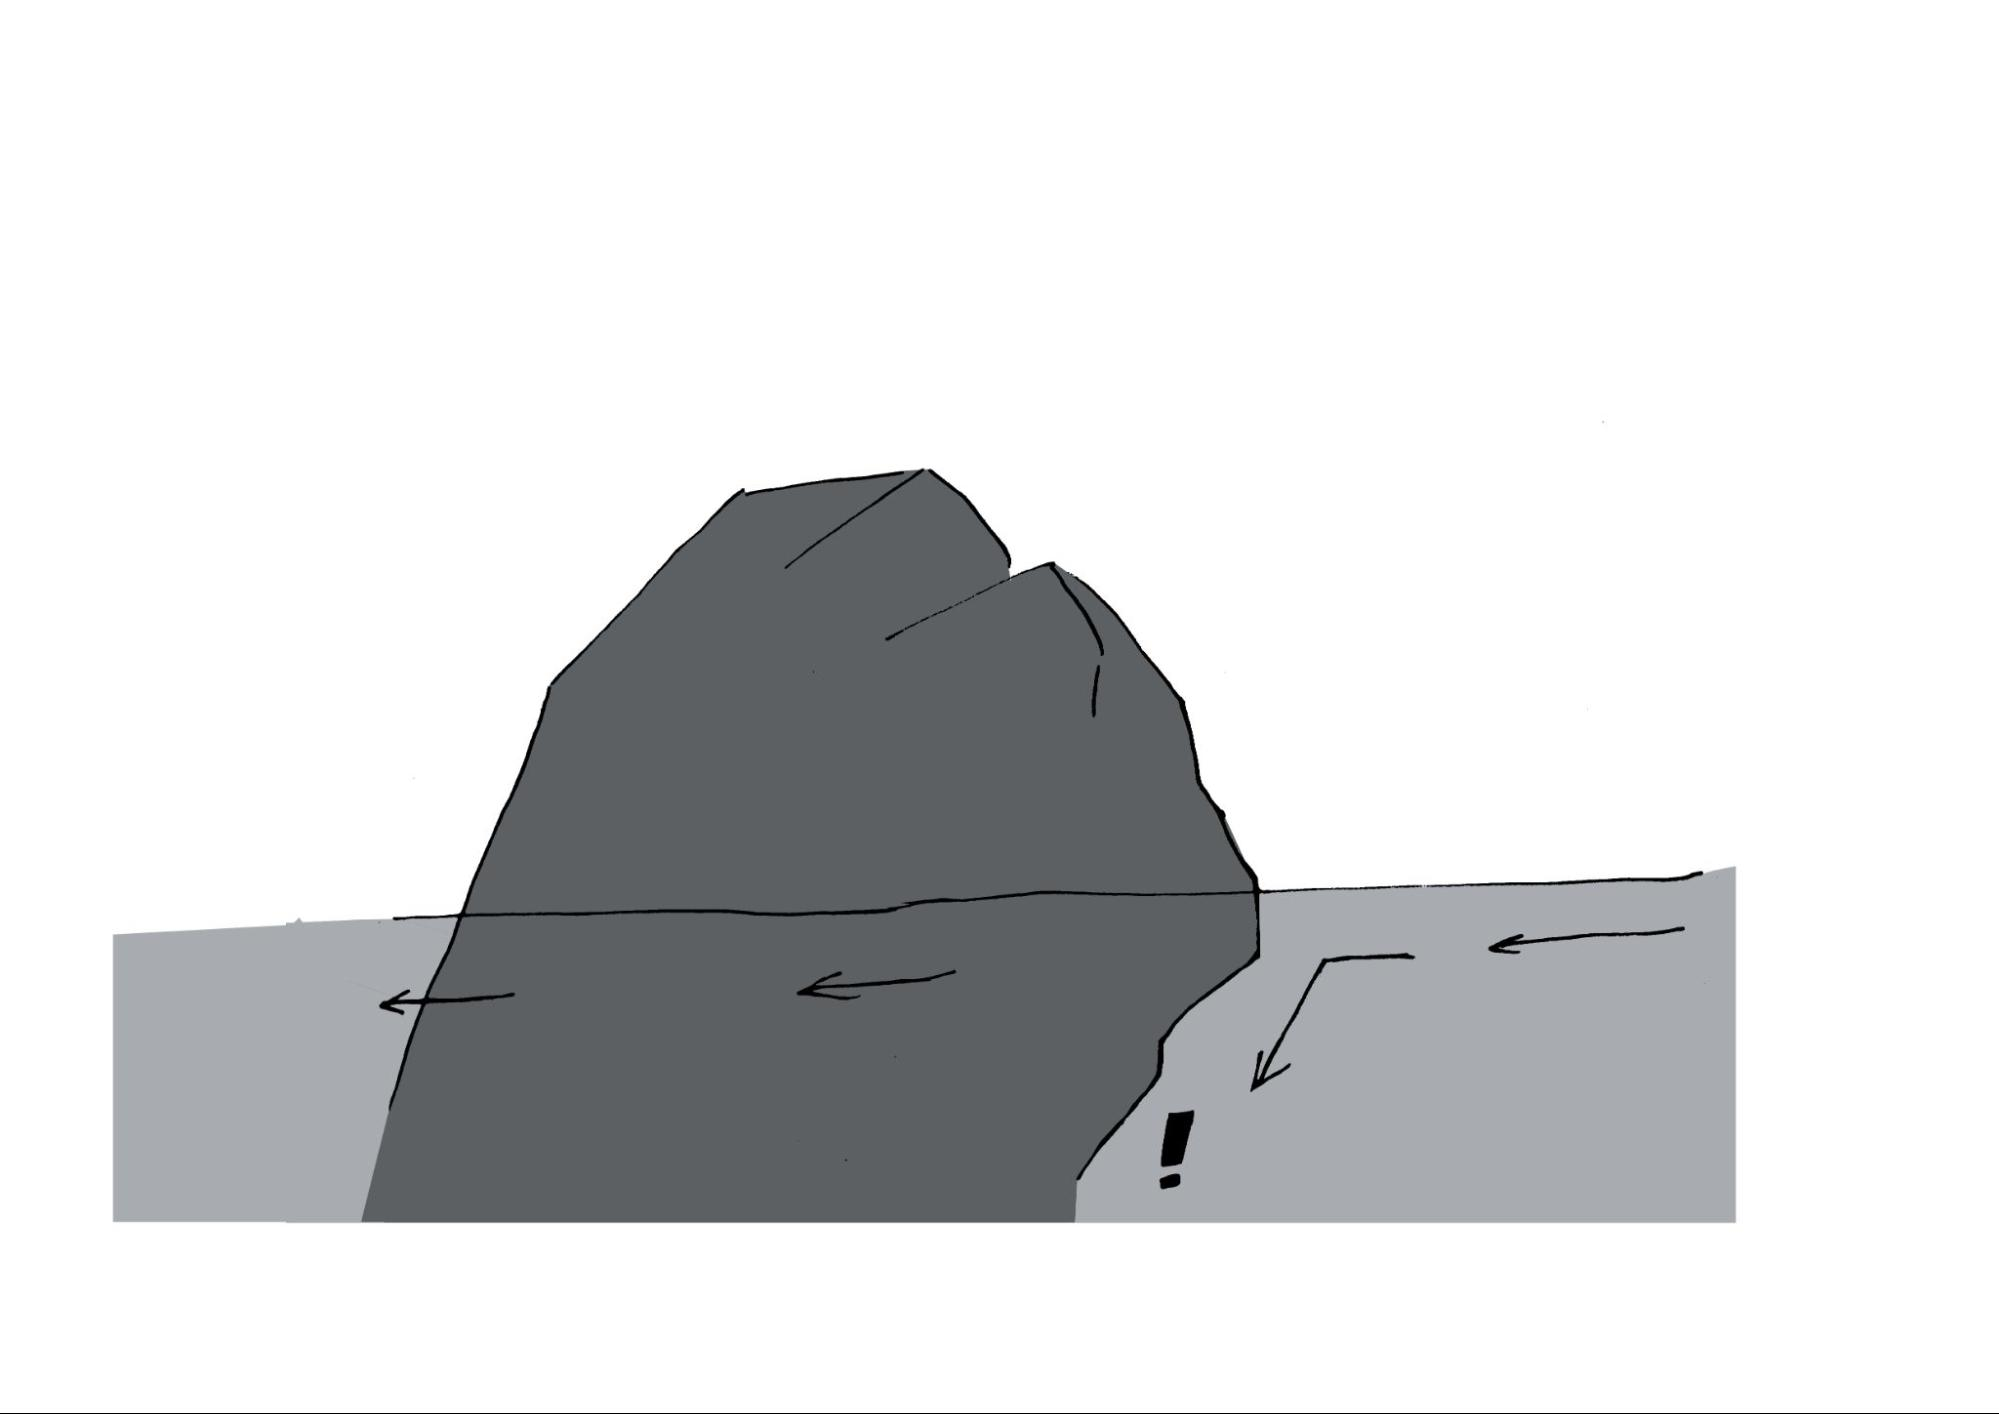
\includegraphics[width=300px]{images/podmytka_syfon.jpg}
    \caption{Wizualizacja podmytki / syfonu}
\end{figure}

\begin{warnbox}
  Podmytki i syfony należą do najbardziej niebezpiecznych przeszkód na rzece górskiej. Zawsze identyfikuj je z brzegu i bezwzględnie omijaj.
\end{warnbox}

% ------------------------------------------------------------
\subsection{Poduszka / Maliniak}
% ------------------------------------------------------------

\textbf{Maliniak} tworzy się, gdy woda wypływająca pionowo (od dna do powierzchni) tworzy charakterystyczny grzybek, na którym kajak może stracić stabilność.

\textbf{Poduszka} to sytuacja, gdzie woda odbija się od kamienia w nurcie — w ten sposób można bezpiecznie rozpoznać kamienie, które dostarczają wiele frajdy doświadczonym kajakarzom.